\documentclass[conference,a4paper]{IEEEtran}
\IEEEoverridecommandlockouts
% The preceding line is only needed to identify funding in the first footnote. If that is unneeded, please comment it out.

\usepackage{cite}
\usepackage{amsmath,amssymb,amsfonts}
\usepackage{algorithmic}
\usepackage{algorithm}
\usepackage{graphicx}
\usepackage{textcomp}
\usepackage{xcolor}
\def\textbi#1{\textbf{\em #1}}
\hyphenpenalty=6000
\tolerance=10000
\ifCLASSOPTIONcompsoc

\usepackage[caption=false,font=normalize,labelfont=sf,textfont=sf]{subfig}
\else
\usepackage[caption=false, font=footnotesize]{subfig}
\def\BibTeX{{\rm B\kern-.05em{\sc i\kern-.025em b}\kern-.08em
    T\kern-.1667em\lower.7ex\hbox{E}\kern-.125emX}}
\begin{document}

\title{A Fog-Aided Privacy-Preserving Truth Discovery Framework over Crowdsensed Data Streams}

\author{\IEEEauthorblockN{Shaoxian Yuan, Bin Zhu, Feng Liu, Jian Li, Kaiping Xue$^\dag$}
\IEEEauthorblockA{School of Cyber Security, University of Science and Technology of China, Hefei, Anhui 230027, China\\
$^\dag$Corresponding author, kpxue@ustc.edu.cn}
}
\maketitle


\begin{abstract}
With the proliferation of mobile and wearable devices, mobile crowdsensing (MCS) is becoming a new paradigm for data collection and analysis. To effectively identify truthful information from crowdsensed data without privacy leakage, privacy-preserving truth discovery (PPTD) has gained much attention recently. Existing works either didn't consider real-time applications over data streams or failed to achieve enough efficiency for a large group of workers. In this paper, we propose FPTD, a Fog-aided Privacy-preserving Truth Discovery framework which is secure and efficient in handling real-time applications with a large group of workers. To reduce overhead, we adopt cloud-fog computing architecture to divide the complete worker group into many smaller ones. Then we design a unique secure aggregation protocol \textbi{SecAgg} which can securely and efficiently aggregate inputs from workers in smaller groups. Finally, we give detailed construction of FPTD, an efficient truth discovery framework based on \textbi{SecAgg} for real-time applications. Through extensive experiments and security analysis, we demonstrate that both \textbi{SecAgg} and FPTD are secure and efficient.
\end{abstract}

\begin{IEEEkeywords}
fog computing, privacy-preserving truth discovery, mobile crowdsensing
\end{IEEEkeywords}

\section{Introduction}\label{intro}
%Generally, instead of treating each worker equally, truth discovery algorithms evaluate each worker's reliability by assigning different $weights$ and compute weighted average values to estimate $truths$.
%For example, data collected for traffic monitoring is likely to reveal worker's location information, which can be misused by third parties and even put workers in danger without protection. Thus, if workers' data privacy cannot be strictly protected, they will resist participating in crowdsensing tasks.

With the rapid advancement and adoption of mobile, wearable and IoT devices, mobile crowdsensing (MCS) is becoming a new paradigm for data collection and analysis. Due to its low deployment cost, wide geographic coverage and flexibility, MCS has enabled a broad range of real-time applications, such as real-time traffic monitoring\cite{trafficapplication}, urban dynamic mining \cite{urbanmining}. In practice, data collected from mobile workers are noisy and unreliable due to background noise and manufacturing quality. In order to identify truthful information from noisy data, many truth discovery algorithms have been proposed \cite{CRH,CATD}. Despite the effectiveness, applying truth discovery to mine truthful information needs to tackle the privacy challenge. In many crowdsensing applications, data records provided by workers may contain sensitive information.


To tackle the privacy challenge, several privacy-preserving truth discovery (PPTD) schemes \cite{miao,rptd,inpptd,rtpt} have been proposed. Generally, they require workers to submit encrypted or masked data records to cloud servers and then perform truth discovery algorithm on encrypted or masked data. However, all these schemes incur limitations in handling real-time applications.

In particular, we address three challenges when designing an efficient PPTD scheme for real-time applications. First, data are collected as streams rather than static datasets in real-time applications. This means that each worker senses and uploads data records at regular intervals. On the one hand, this challenge requires a streaming truth discovery algorithm underlying PPTD scheme. On the other hand, it requires that the PPTD scheme should be able to report an estimation at regular intervals. Second, workers in real-time applications are dynamic. Workers in real-time applications may drop out at any time due to various reasons such as disconnection of network, unexpected termination of mobile device ,etc. This challenge requires the PPTD scheme to be failure robust, i.e., output correct estimation even if some workers drop out. Third, the number of workers may vary in scale. For large-scale real-time applications like dynamic mining, any mobile user could be a worker to contribute his/her social recording to earn some profits. This requires that PPTD scheme should be efficient even if the number of workers grows dramatically.

Roughly speaking, the majority of existing works \cite{miao,rptd,inpptd} only focus on static data. Other work such as \cite{rtpt} is able to overcome the first two challenges while overlooking the third one, resulting in inefficiency with respect to a large group of workers. To be specific, the inefficiency of \cite{rtpt} is caused by the underlying secure aggregation protocol, called double masking \cite{doublemasking}. For a large group of workers, double masking requires each worker to maintain a connection with every other worker to ensure privacy preservation. However, we argue that each worker maintaining connections with a much smaller group is enough to ensure privacy.

%Specifically, we introduce fog nodes under a cloud server and then assign different workers to different fog nodes. This directly breaks the complete worker group into many smaller groups. Then we design a secure aggregation protocol which can securely aggregate inputs from these small groups without revealing any extra information except the aggregation result.

%which requires each worker to maintain a connection with every other worker without considering the fact that the complete worker group can be large at scale. However, we demonstrate that each worker maintaining connections with a smaller group of other workers is enough to ensure the privacy of each worker's input.

%However, trivial solution that each fog node securely aggregate inputs from assigned workers individually then cloud server aggregates intermediate values from fog nodes poses privacy breach. The reason is that the trivial solution not only outputs the aggregation result but also reveals the intermediate values, which leaks extra information to adversary.

In particular, our contributions can be summarized below:
\begin{itemize}
  \item First, we turn to cloud-fog computing architecture to divide the complete worker group into many smaller ones. In this way, we require each worker maintain connections with only its neighbours in the same group. This significantly reduces the number of connections each worker has to maintain.
  \item Second, we design a novel failure-robust secure aggregation protocol \textbi{SecAgg} which can securely aggregate inputs from all small worker groups efficiently.
  \item Finally, we give a detailed construction of FPTD framework based on \textbi{SecAgg} for real-time applications in MCS. Moreover, through extensive experiments and security analysis, we demonstrate that our FPTD is secure and efficient for real-time applications in MCS.
\end{itemize}

The remainder of this paper is organized as follows. In section \ref{relatedwork}, we review existing works of PPTD. The system model and threat assumption are given in section \ref{problem_state}. In section \ref{prel}, we describe the underlying truth discovery algorithm and cryptographic primitives we adopt. In section \ref{scheme}, we introduce the proposed scheme in detail. In section \ref{sec_analysis}, we give security proof. Afterwards, performance evaluation is given in section \ref{performance}. Finally, we conclude our paper in section \ref{conclusion}.

\section{Related Work}\label{relatedwork}
The majority of existing works \cite{miao,rptd,inpptd} focus on PPTD over static data. The first work of PPTD was presented by \cite{miao}, which adopted threshold Paillier cryptosystem under a single cloud server. However, \cite{miao} introduced heavy computation burdens over both workers and cloud server. To optimize the performance, \cite{rptd} utilized an improved Paillier cryptosystem and super-increasing sequence under the cloud-fog computing architecture. \cite{inpptd} realized a PPTD with an incentive mechanism to resist potential lazy workers by reducing the reward a lazy worker can obtain. However, existing PPTD work on static data cannot naturally extend to real-time applications due to the heavy cryptographic tools they adopt.

To address real-time applications, \cite{rtpt} adopted a lightweight secure aggregation protocol to realize PPTD which can support worker's dropout. Besides, \cite{rtpt} exploited a steaming truth discovery to efficiently identify truths from data streams. These two unique designs helps \cite{rtpt} overcome the first two challenges while overlooking the third one. Though some more lightweight aggregation protocol \cite{gai} based on differential privacy can help overcome the third challenge, the security would be degraded.

\section{Problem Statement}\label{problem_state}
    \subsection{System Model}
    Our system is a cloud-fog computing architecture. It consists of three entities: cloud server, fog nodes and workers. The cloud server is a remote server provided by a cloud service provider. Fog nodes are at the edge of network and close to workers. Workers can be devices with different sensors, such as smart phones, wearable and IoT devices. Cloud server maintains a connection with fog nodes and each fog node manages a group of workers. Fog nodes relay the messages between any two workers or workers and the cloud server. Formally, we assume there are $M$ objects to be sensed $\mathcal{M}=\{o_1,\cdots,o_M\}$ and $K$ fog nodes $\mathcal{F}=\{f_1,\cdots,f_K\}$. Each fog node $f_u$ manages $n_u$ workers $\mathcal{S}_u=\{s_1,s_2,\cdots,s_{n_u}\}$. In each time slot $t$, each worker collects data record $\textbi{x}_i^t=\{x_i^{m,t}\}_{m=1}^M$, updates distance $d_i^t$ and weight $w_i^t$. Estimated truth is represented as $\textbi{x}_t^*=\{x_{m,t}^*\}_{m=1}^M$.


    \subsection{Threat Model}
     Similar to other PPTD works, we consider a semi-honest adversary where both fog nodes and cloud server faithfully behave as the protocol requires, while they try to infer private information from transcripts in the meantime. We also assume workers are honest because they are stimulated by incentives \cite{theseus} which is another important topic in MCS.

     In this paper, we build the security of \textbi{SecAgg} on the common assumption that no fog nodes will collude with the cloud server.


    \subsection{Design Goals}
    % 这部分的内容应该在security analysis和performance evaluation中提到或证明,即要能够证明达到了设计目标
    % 就写达到了什么具体的性质,而不是具体的工作。
    Our design goals are three folds.

    %这个可以在correctness说明,即便有用户退出,也可以输出正确的结果
    {\em Failure-robustness}. The proposed FPTD framework should output correct estimation based on the remaining workers' sensory data even if some workers may drop out unexpectedly like \cite{rtpt}.

    %这个可以通过实验来证明
    {\em Efficiency}. The proposed FPTD should reach significantly lower overheads for both workers and cloud server compared with \cite{rtpt}.

    %这个可以通过安全性分析来证明
    {\em Security}. We require the proposed FPTD can securely perform the process of truth discovery to identify truths from workers' noisy sensory data without revealing any data and weights.


\section{Preliminaries}\label{prel}
    In this section, we will illustrate the underlying truth discovery algorithm and cryptographic primitives.
    \subsection{Truth Discovery}
    The underlying truth discovery algorithm we adopt is the incremental CRH (iCRH) \cite{CRH}. The basic idea behind iCRH is to assign a $weight$ to each worker to measure reliability and aggregate weighted average to obtain estimated $truth$.

    The iCRH handles data streams. In each time slot $t$, iCRH is divided into three steps: truth update, distance update and weight update.
    \begin{itemize}
        \item Truth update: In this step, given each worker's sensory data $\textbi{x}_i^t$ and weight $w_i^{t-1}$ of last time slot, estimation of truth is updated as a weighted average
            \begin{equation}\label{icrh-truth}
                \textbi{x}_t^*=\frac{\sum_{i=1}^{S} w_i^{t-1} \times \textbi{x}_i^t}{\sum_{i=1}^{S} w_i^{t-1}}.
            \end{equation}
        \item Distance update: In this step, each worker updates their incremental distances $d_i^t$ as below, given estimated truth, sensory data and previous distance $d_i^{t-1}$
            \begin{equation}\label{icrh-distance}
                d_i^t=\alpha\times d_i^{t-1}+d(\textbi{x}_i^t, \textbi{x}_t^*),
            \end{equation}
            where distance function $d(\textbi{x},\textbi{y})$ measures the deviation level of two sensory data records of dimension $M$. For continuous data, we have $d(\textbi{x},\textbi{y})=\sum_{m=1}^{M} (x_i^{m,t}-y_i^{m,t})^2$ and for categorial data, $d(\textbi{x},\textbi{y})=\sum_{m=1}^{M} \textbf{1}(x_i^{m,t},y_i^{m,t})$ where $\textbf{1}(x,y)=1$ if $x\ne y$ and 0 otherwise. Besides, $\alpha$ represents decay rate to allow more recent data to play more important role.
        \item Weight update: In this step, given each worker's distance, each worker's weight is updated as
            \begin{equation}\label{icrh-weight}
                w_i^t=\log (\sum_{i=1}^{S} d_i^t)-\log (d_i^t).
            \end{equation}
    \end{itemize}
    \subsection{Key Agreement}
    The key agreement  establishes secrets between workers. It consists of three algorithms:
    $\mathbf{KA.param}$,$\mathbf{KA.gen}$ and $\mathbf{KA.agree}$.
    \begin{itemize}
        \item $\mathbf{KA.param}(1^\lambda)\mapsto (\mathbb{G},g,p)$: Taking security parameter $\lambda$ as input, the algorithm outputs public parameters $pp$.
        \item $\mathbf{KA.gen}(pp)\mapsto (c_i^{PK},c_i^{SK})$: Taking the input of $pp$, the algorithm returns a public key pair to any worker $i$.
        \item $\mathbf{KA.agree}(c_i^{SK},c_j^{PK})\mapsto sc_{i,j}$: Given the secret key of $s_i$ and the public key of $s_j$, the algorithm returns a shared key.
    \end{itemize}

    For correctness, we require that $\forall i\ne j$, $\mathbf{KA.agree}(c_i^{SK},c_j^{PK})=\mathbf{KA.agree}(c_j^{SK},c_i^{PK})=sc_{ij}$. For security, we rely on Decisional Diffle-Hellman assumption (DDH) \cite{DDH}.

    \subsection{Secret Share}
    We rely on Shamir's $t$-out-of-$n$ secret share \cite{shamir}, which allows someone to split a secret $s$ into $n$ shares, such that any $t$ shares can be used to reconstruct $s$, but any set of at most $t-1$ shares gives no information about $s$.

    Specifically, sharing algorithm $\mathbf{SS.share}(s,t,\mathcal{U})\mapsto \{(i,s_i)\}_{i\in\mathcal{U}}$ takes as input a secret $s$, a set $\mathcal{U}$ of $n$ workers, and a threshold $t\le |\mathcal{U}|$. For correctness, we require $\forall s,t,n$ with $1\le t\le n$, $\forall |\mathcal{U}|=n$ if $\mathbf{SS.share}(s,t,\mathcal{U})\mapsto \{(i,s_i)\}_{i\in\mathcal{U}}$, for $\mathcal{V}\subseteq \mathcal{U}$ and $|\mathcal{V}|\ge t$, then $\mathbf{SS.rec}(\{j,s_j\}_{j\in\mathcal{V}},t)=s$.

\section{Proposed Scheme}\label{scheme}
    \subsection{Overview}
    % a brief about double masking
    % why double masking and trivial solution fails
    % re-mask technique
    % FPTD construction
    %Note that our work consists of two components: \textbi{SecAgg} and construction of FPTD. To illustrate \textbi{SecAgg} clearly, we first briefly review double masking and demonstrate that trivially applying double masking is insecure. After that, we show how to transform double masking into a secure aggregation protocol \textbi{SecAgg} via a re-mask technique. Finally, we give construction of FPTD based on \textbi{SecAgg}.

    Double masking is a failure-robust secure aggregation protocol under the single server model. It employs two layers of masks to protect workers' inputs. Generally, the first layer is a zero-sum mask which can be canceled if no worker drops out. The second layer is a random mask which can only be removed by recovering the seeds. To handle workers' dropouts, double masking exploits $t$-out-of-$n$ Shamir's secret sharing to distribute the secrets among all workers, which can help the central server to recover the two masks. Trivially applying double masking within each small group poses privacy breach since trivial solution not only outputs the final sum of inputs from all workers but also reveals partial sums of each group, which leaks extra information to a potential adversary.

    We transform double masking to \textbi{SecAgg} via a re-mask technique. Our idea consists of two steps. First, similar to the trivial solution, we require each worker to add two layers of masks. However, we let each fog node remove the zero-sum mask and leave the random mask to the cloud server. Besides, we require each fog node adds one layer of the zero-sum mask to the intermediate value to preserve privacy against the cloud server.

    After transforming double masking to \textbi{SecAgg}, we construct the secure truth update and secure weight update for FPTD. Our construction is quite simple and straight. We utilize \textbi{SecAgg} to aggregate weights and weighted truths to update truths according to equation \ref{icrh-truth}. Similarly, we aggregate distance information from all workers to update weights according to equation \ref{icrh-weight}.

    \subsection{\textbf{SecAgg}}\label{sec_sum}
    We observe that even though workers are dynamic and may drop out at any time, fog nodes are relatively stable and can maintain a long-term connection with the cloud server. Therefore we can avoid secret sharing among fog nodes which saves computation and communication.

    Assume $n=\sum_{u=1}^U n_u$ represents the number of all workers and worker's id $i\in [n]$. Let $S$, $s_i$ and $f_u$ represent the cloud server, the $u$-th fog node and worker $i$ respectively. Then we define $G(i,j)=1$ if $s_i$ and $s_j$ are in same $\mathcal{S}_u$ managed by $f_u$, 0 otherwise. In particular, $\forall$ $i\in [n], G(i,S)=1$ holds. To support worker's dropout, the threshold for each small group is defined $t_u=\lceil \frac{3}{4} n_u\rceil$. We also assume each worker holds a vector $\textbi{x}_i$ of dimension $M^\prime$.\\

    {\em Round 0: One Time Initialization.}
    In this round, \textbi{SecAgg} establishes long-term keys between workers and the cloud server. First, $S$ generates public parameters $pp$ which is a cyclic group $\mathbb{G}$ with prime order $p$ and generator $g$ via
    \begin{equation}\nonumber
        \textbf{KA.param}(1^\lambda)\mapsto (\mathbb{G},p,g).
    \end{equation}
    Then $S$ publishes $pp$ to all fog nodes and  workers. After obtaining $pp$, each $s_i$ including $S$ generates a key pair
    \begin{equation}\nonumber
      \textbf{KA.gen}(pp)\mapsto (c_i^{PK},c_i^{SK}),
    \end{equation}
    where $i\in [n]\cup \{S\}$. After key generation, each $s_i$ exchanges $(i,c_i^{PK})$ with every other $s_j$ if $G(i,j)=1$. Besides, $S$ exchanges $(S,c_S^{PK})$ with every $s_i$. After the exchange, each $s_i$ establishes key
    \begin{equation}\nonumber
      sk_{i,j}=\textbf{KA.agree}(c_i^{SK},c_j^{PK}),
    \end{equation}
    where $j\in [n]\cup {S}/\{i\}$ and $G(i,j)=1$. Likewise, $S$ establishes keys $sk_{i,S}$ $\forall$ $i\in [n]$. These keys serve as the keys for symmetric Authenticated Encryption, i.e. \textbf{AE}.\\

    {\em Round 1: Establish Zero-Sum Seeds.} After one time initialization, both workers and fog nodes need to establish shared seed to generating zero-sum masks. Specifically, each $s_i$ and $f_u$ generates new key pairs
    \begin{equation}\nonumber
    \begin{aligned}
      &\textbf{KA.gen}(pp)\mapsto (s_i^{PK},s_i^{SK}),\\
      &\textbf{KA.gen}(pp)\mapsto (z_u^{PK},z_u^{SK}),
    \end{aligned}
    \end{equation}
    where $i,j\in [n]$ and $u,v\in [K]$. Then each $s_i$ exchanges $(i,s_i^{PK})$ with every $s_j$ where $G(i,j)=1$ and each fog node exchanges $(u,z_u^{PK})$ with every $f_v$. Afterwards, each $s_i$ and $f_u$ establishes shared secrets
    \begin{equation}\nonumber
    \begin{aligned}
      &s_{i,j}=\textbf{KA.agree}(s_i^{SK},s_j^{PK}),\\
      &z_{u,v}=\textbf{KA.agree}(z_u^{SK},z_v^{PK}),
    \end{aligned}
    \end{equation}
    respectively.\\

    {\em Round 2: Share Secrets.}
    In this round, each $s_i$ shares his/her random seed and secret key within his/her group. Besides, each fog node $f_u$ shares his/her secret key with all other fog nodes. First, each $s_i$ first uniformly samples random seed $r_i$ for random masks. Then each $s_i$ divides $s_i^{SK}$, $r_i$ into shares via
    \begin{equation}\nonumber
    \begin{aligned}
      &\textbf{SS.share}(s_i^{SK},t_u)\mapsto &\{(j,s_{i,j}^{SK})\}_{j\in \mathcal{S}_u/\{i\}},\\
      &\textbf{SS.share}(r_i,t_u)\mapsto &\{(j,r_{i,j})\}_{j\in \mathcal{S}_u/\{i\}},
    \end{aligned}
    \end{equation}
    where $G(i,j)=1$. After dividing shares, each $s_i$ encrypts the shares
    \begin{equation}\nonumber
    \begin{aligned}
        &e_{i,j}=\textbf{AE.encrypt}(sk_{i,j},i||j||s_{i,j}^{SK}||r_{i,j}),\\
    \end{aligned}
    \end{equation}
    then each $s_i$ exchanges $e_{i,j}$ with $s_j$ where $j\in [n]$ and $G(i,j)=1$.\\

    {\em Round 3: Masked Input Collection.} In this round, each $s_i$ generates random mask $\textbi{b}_i$ and zero-sum mask $\textbi{s}_{i,j}$. For each $m\in [M^\prime]$, $s_i$ computes each element
    \begin{equation}\nonumber
    \begin{aligned}
      b_i^m=&H(r_i||m) \mod{p},\\
      s_{i,j}^m=&H(s_{i,j}||m) \mod{p},
    \end{aligned}
    \end{equation}
    where $H$ is a cryptographic hash function. Then $s_i$ adds masks to input
    \begin{equation}\nonumber
    \begin{aligned}
        \textbi{y}_i=\textbi{x}_i&+\textbi{b}_i\\
                                 &+\sum_{j\in \mathcal{S}_u/\{i\}:i>j} \textbi{s}_{i,j}\\
                                 &-\sum_{j\in \mathcal{S}_u/\{i\}:i<j} \textbi{s}_{i,j}\mod{p}.
    \end{aligned}
    \end{equation}
    and sends masked input $\textbi{y}_i$ to corresponding fog node $f_u$.\\

    {\em Round 4: Re-Mask.} Assume some workers drop out before sending the masked inputs and we use $\mathcal{S}_u^\prime$ to represent the surviving workers. Upon receiving masked inputs from surviving workers, $f_u$ aggregates
    \begin{equation}\label{aggregate1}
    \begin{aligned}
        \sum_{i\in \mathcal{S}_u^\prime} \textbi{y}_i
        &=\sum_{i\in \mathcal{S}_u^\prime} \left( \textbi{x}_i+\textbi{b}_i+\sum_{j\in \mathcal{S}_u/\{i\}:i>j} \textbi{s}_{i,j}-\sum_{j\in \mathcal{S}_u/\{i\}:i<j} \textbi{s}_{i,j}\right)\\
        &=\sum_{i\in \mathcal{S}_u^\prime}\left(\textbi{x}_i+\textbi{b}_i\right)+\sum_{i\in\mathcal{S}_u}\sum_{j\in \mathcal{S}_u/\mathcal{S}_u^\prime:i>j}\textbi{s}_{i,j}\\
        &\quad\qquad\qquad\qquad-\sum_{i\in\mathcal{S}_u}\sum_{j\in \mathcal{S}_u/\mathcal{S}_u^\prime:i<j}\textbi{s}_{i,j}.
    \end{aligned}
    \end{equation}
    To recover $\sum_{i\in \mathcal{S}_u^\prime}\left(\textbi{x}_i+\textbi{b}_i\right)$, each fog node $f_u$ sends $\mathcal{S}_u^\prime$ to surviving workers and request $\{s_{i,j}^{SK}\}_{i\in \mathcal{S}_u/\mathcal{S}_u^\prime}$ from workers in $\mathcal{S}_u^\prime$. After receiving shares from surviving workers, each fog recovers the secret key via $\textbf{SS.rec}$. Then $f_u$ recovers the missing zero-sum masks and adds them to equation \ref{aggregate1} to obtain the randomly masked input.

    Afterwards, each $f_u$ generates the new zero-sum mask. For each $m\in [M^\prime]$, $f_u$ computes
    \begin{equation}\nonumber
      z_{u,v}^m=H(z_{u,v}||m)\mod{p},
    \end{equation}
    then $f_u$ computes
    \begin{equation}\nonumber
      \textbi{z}_u=\sum_{i\in \mathcal{S}_u^\prime} \left(\textbi{x}_i+\textbi{b}_i\right)+\sum_{v\in \mathcal{F}:u>v} \textbi{z}_{u,v}-\sum_{v\in \mathcal{F}:u<v} \textbi{z}_{u,v}.
    \end{equation}
    Finally, $f_u$ sends $z_u$ to cloud server.\\

    {\em Round 5: Unmasking.}
    After receiving $\textbi{z}_u$ from all fog nodes, $S$ computes
    \begin{equation}\nonumber
    \begin{aligned}
      C_{agg}&=\sum_{u\in \mathcal{F}} \left(\sum_{i\in \mathcal{S}_u^\prime} \left(\textbi{x}_i+\textbi{b}_i\right)+\sum_{v\in \mathcal{F}:u>v} \textbi{z}_{u,v}-\sum_{v\in \mathcal{F}:u<v} \textbi{z}_{u,v}\right)\\
             &=\sum_{u\in \mathcal{F}} \sum_{i\in \mathcal{S}_u^\prime} \left(\textbi{x}_i+\textbi{b}_i\right)+\sum_{u\in \mathcal{F}}\sum_{v\in\mathcal{F}} \textbi{z}_{u,v}-\sum_{u\in \mathcal{F}}\sum_{v\in\mathcal{F}} \textbi{z}_{u,v}\\
             &=\sum_{u\in \mathcal{F}} \sum_{i\in \mathcal{S}_u^\prime} \left(\textbi{x}_i+\textbi{b}_i\right)
    \end{aligned}
    \end{equation}
    In order to remove the random mask, the cloud server requests $r_{j,i}$ from each $s_i$. Then each worker $s_i$ encrypts the secret share
    \begin{equation}\nonumber
      D_{i,j}=\textbf{AE.encrypt}(sk_{i,S},j||i||r_{j,i})
    \end{equation}
    and sends the list $\{D_{i,j}\}_{j\in \mathcal{S}_u^\prime}/\{i\}$ to $S$ through $f_u$. Upon receiving encrypted secret shares from all surviving workers, $S$ decrypts them and recover all $r_i$, then generates random masks to obtain the aggregation result $\sum_{u\in \mathcal{F}} \sum_{i\in \mathcal{S}_u^\prime} \textbi{x}_i$.
\addtolength{\leftmargin}{0.584cm}

    \subsection{FPTD Construction}
    In this part, we give detailed construction of FPTD. Note that the plaintext numbers are float while cryptographic primitives are performed on integers. We use a rounding factor of $10^6$ to scale float numbers up to integers.
        \subsubsection{Initialization}
        Before collecting and transmitting data, each worker $s_i$ initializes their weight as $w_i^0=1$ and distance as $d_i^0=0$. Then $S$ initializes the public parameters and establishes symmetric keys via {\em One Time Initialization}.
        \subsubsection{Secure Truth Update}
        In this phase, FPTD securely aggregates weights and weighted truths to update the truths according to equation \ref{icrh-truth}. In each time slot $t$, each $s_i$ first collects sensory data $\textbi{x}_i^t$ and uploads his weight $w_i^{t-1}$ and weighted truth $w_i^{t-1}\times \textbi{x}_i$ via \textbi{SecAgg}. Notice that we can concatenate both values into one vector $\langle w_i^{t-1}\times \textbi{x}_i,w_i^{t-1}\rangle$, resulting in only one call to \textbi{SecAgg}.
        \subsubsection{Secure Weight Update}
        In this phase, $S$ first returns truths $\textbi{x}_t^*$ to all workers. After receiving truths, each $s_i$ first updates his distance according to equation \ref{icrh-distance} to obtain $d_i^t$. Then each worker submits his distance to $S$ via \textbi{SecAgg}. After obtaining aggregated distance $\sum_{u\in \mathcal{F}} \sum_{i\in \mathcal{S}_u^\prime} d_i^t$, $S$ computes $\log{(\sum_{u\in \mathcal{F}} \sum_{i\in \mathcal{S}_u^\prime} d_i^t)}$ and returns it to all workers. Upon receiving $\log{(\sum_{u\in \mathcal{F}} \sum_{i\in \mathcal{S}_u^\prime} d_i^t)}$, each worker updates his weight according to equation \ref{icrh-weight}.\\

    After initialization, FPTD executes Secure Truth Update phase and Secure Weight Update phase once in each time slot $t$.
\section{Security Analysis}\label{sec_analysis}
    \textbf{Theorem 1.}  {\em Suppose there is at least one group and each group contains at least 3 workers providing different sensory data for each object. If all entities are semi-honest and there is no collusion between fog nodes and cloud server, the sensory data and weight will not be disclosed to any other entity under FPTD framework.}

    {\em proof.} In order to prove that FPTD is secure, we only need to prove the proposed \textbi{SecAgg} is secure. There are three types of attacks an adversary can potentially launch under the semi-honest assumption.

    First, an adversary can compromise fog nodes. Once the adversary compromises some fog nodes $\mathcal{F}_c\subset \mathcal{F}$, he/she can obtain the combined view of these fog nodes which is a list $\{\sum_{i\in \mathcal{S}_u^\prime}\textbi{x}_i+\textbi{b}_i\}_{u\in \mathcal{F}_c}$. However, since the random seeds used to recover the random masks are encrypted using the symmetric keys established between workers and the cloud server, the adversary is not able to recover any $\textbi{x}_i$ or any partial result.

    Second, an adversary can compromise the cloud server. Once the adversary compromises cloud server, he/she can remove all random masks and obtain both $\sum_{i\in\mathcal{S}_u^\prime}\textbi{x}_i+\sum_{v\in\mathcal{F}:u>v}\textbi{z}_{u,v}-\sum_{v\in\mathcal{F}:u<v}\textbi{z}_{u,v}$ for each $f_u$ and $\sum_{u\in\mathcal{F}}\sum_{i\in\mathcal{S}_u^\prime}\textbi{x}_i$. However, since we assume no collusion between fog nodes and the cloud server, the cloud server cannot remove the zero-sum masks added by each fog node, therefore cloud server can only obtain aggregation result $\sum_{u\in\mathcal{F}}\sum_{i\in\mathcal{S}_u^\prime}\textbi{x}_i$.

    Finally, collusion may happen between workers or fog nodes. Collusion in each group under the threshold $t_u$ reveals nothing to corrupted workers since a $t$-out-of-$n$ Shamir's secret sharing is information-theoretically secure against up to $t-1$ corrupted parties.


\section{Performance Analysis}\label{performance}
    Here we conduct the performance comparison between our scheme and \cite{rtpt} in terms of computation overhead and communication overhead.
    % 陈述实验环境
    The simulation is built using a PC with 3.60Ghz Intel i7 and 16GB RAM running Windows 10. FPTD is implemented in Python. Specifically, we construct key agreement protocol from Elliptic-Curve over the NIST P-256 curve composed with SHA256, authenticated encryption from AES-GCM with a 128-bit key. In addition, we also implement \cite{rtpt} as a baseline scheme for comparison.
    % 陈述测试集从哪里获得
    Without loss of generality, we generate a dataset by sampling random numbers as ground truths and add different levels of Gaussian noise to simulate different levels of reliability of workers in MCS applications. Notice that, we regard a worker's reliability in different time slots as a dynamic variable since the ground truths for each object are rapidly changing over time.

     For clarity, we present each entity's overhead in one time slot which consists of a {\em Secure Truth Update} and a {\em Secure Weight Update}. Besides we execute each experiment 50 times and present the average. Specifically, we assume the complete worker group is divided into groups equally. By default, we set the number of workers as 300, the number of fog nodes as 5, the number of objects as 100 and the drop rate as 0.05.

    \subsection{Computation}
    First, we consider varying number of workers which varies from 100 to 500 by the stride of 50.  As shown in Fig.\ref{workers}, with the increasing number of workers, FPTD achieves better efficiency with respect to workers, fog and cloud. In particular, cloud computation overhead of \cite{rtpt} grows to be unacceptable when the number reaches 500 since the computation cost is beyond 30 minutes.
    \begin{figure}[!ht]
        \centering
        \subfloat[Average time of workers]{
        \label{workers_a}
        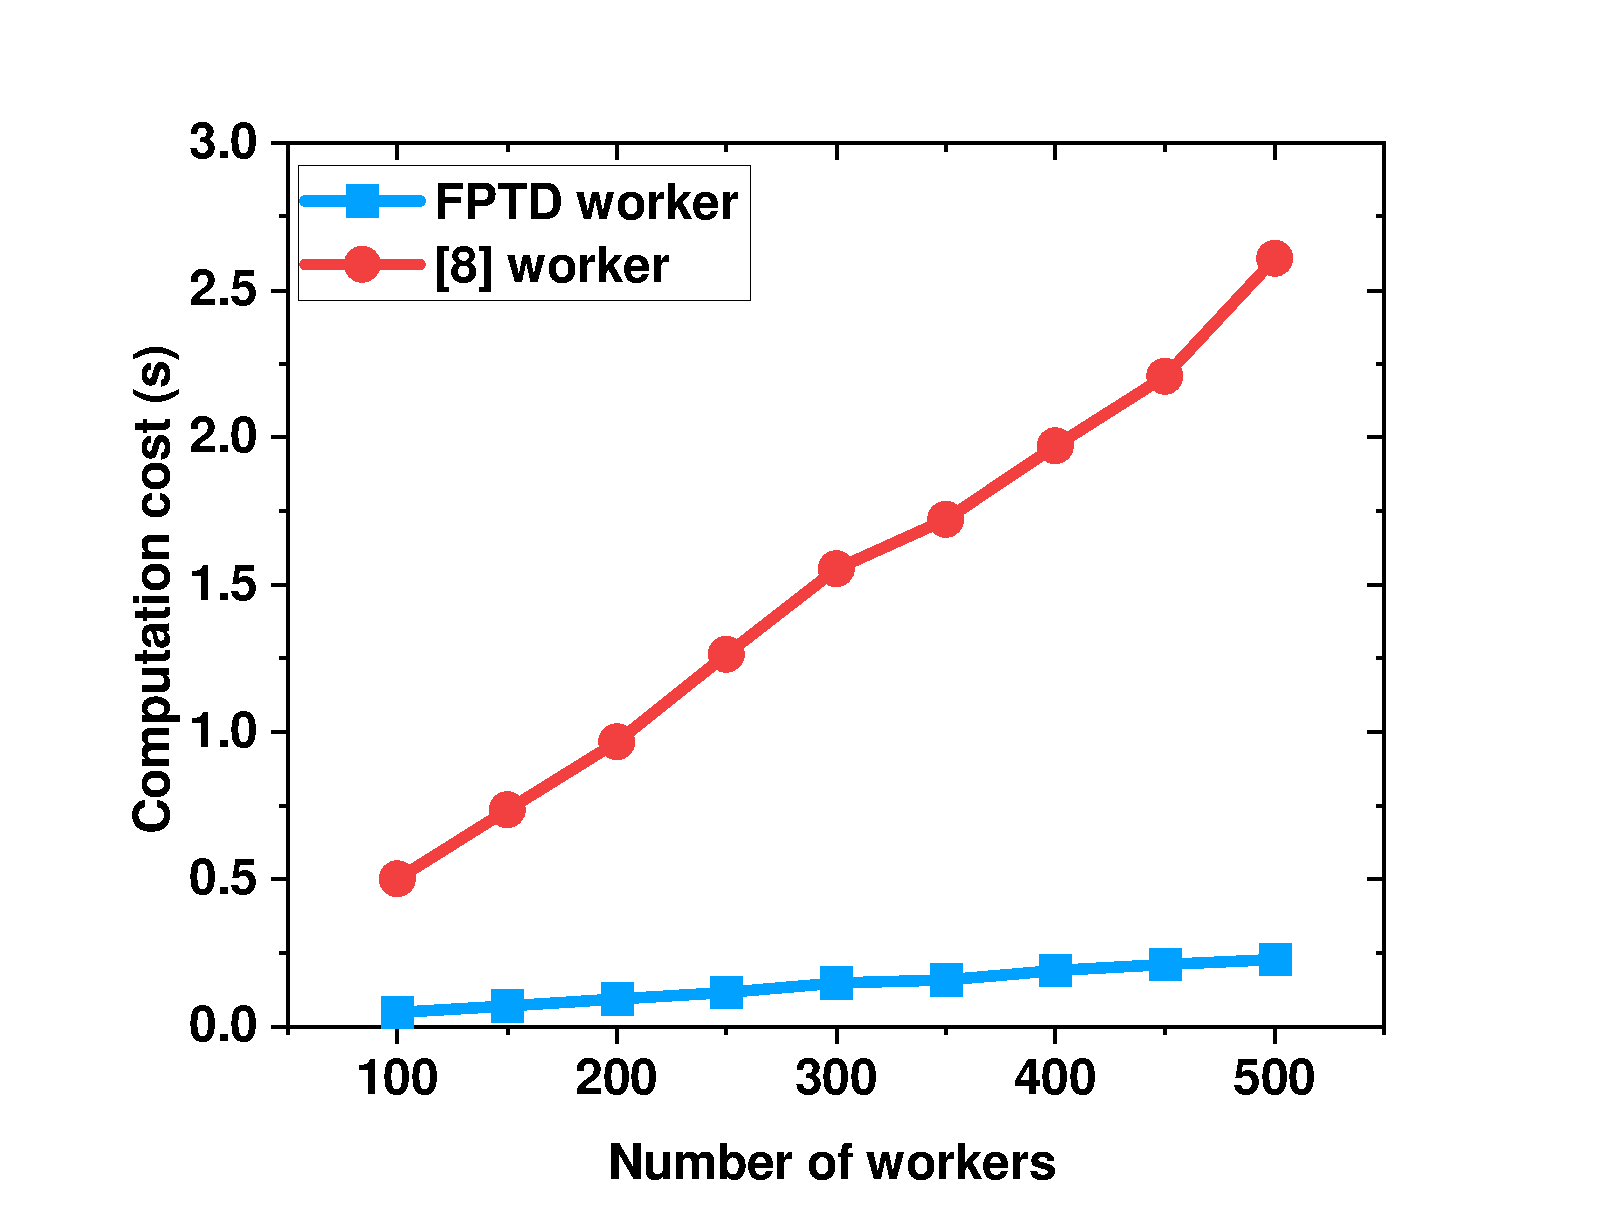
\includegraphics[width=0.48\linewidth]{pictures/varying_workers_worker.pdf}}
        \subfloat[Average time of cloud and fog]{
        \label{workers_b}
        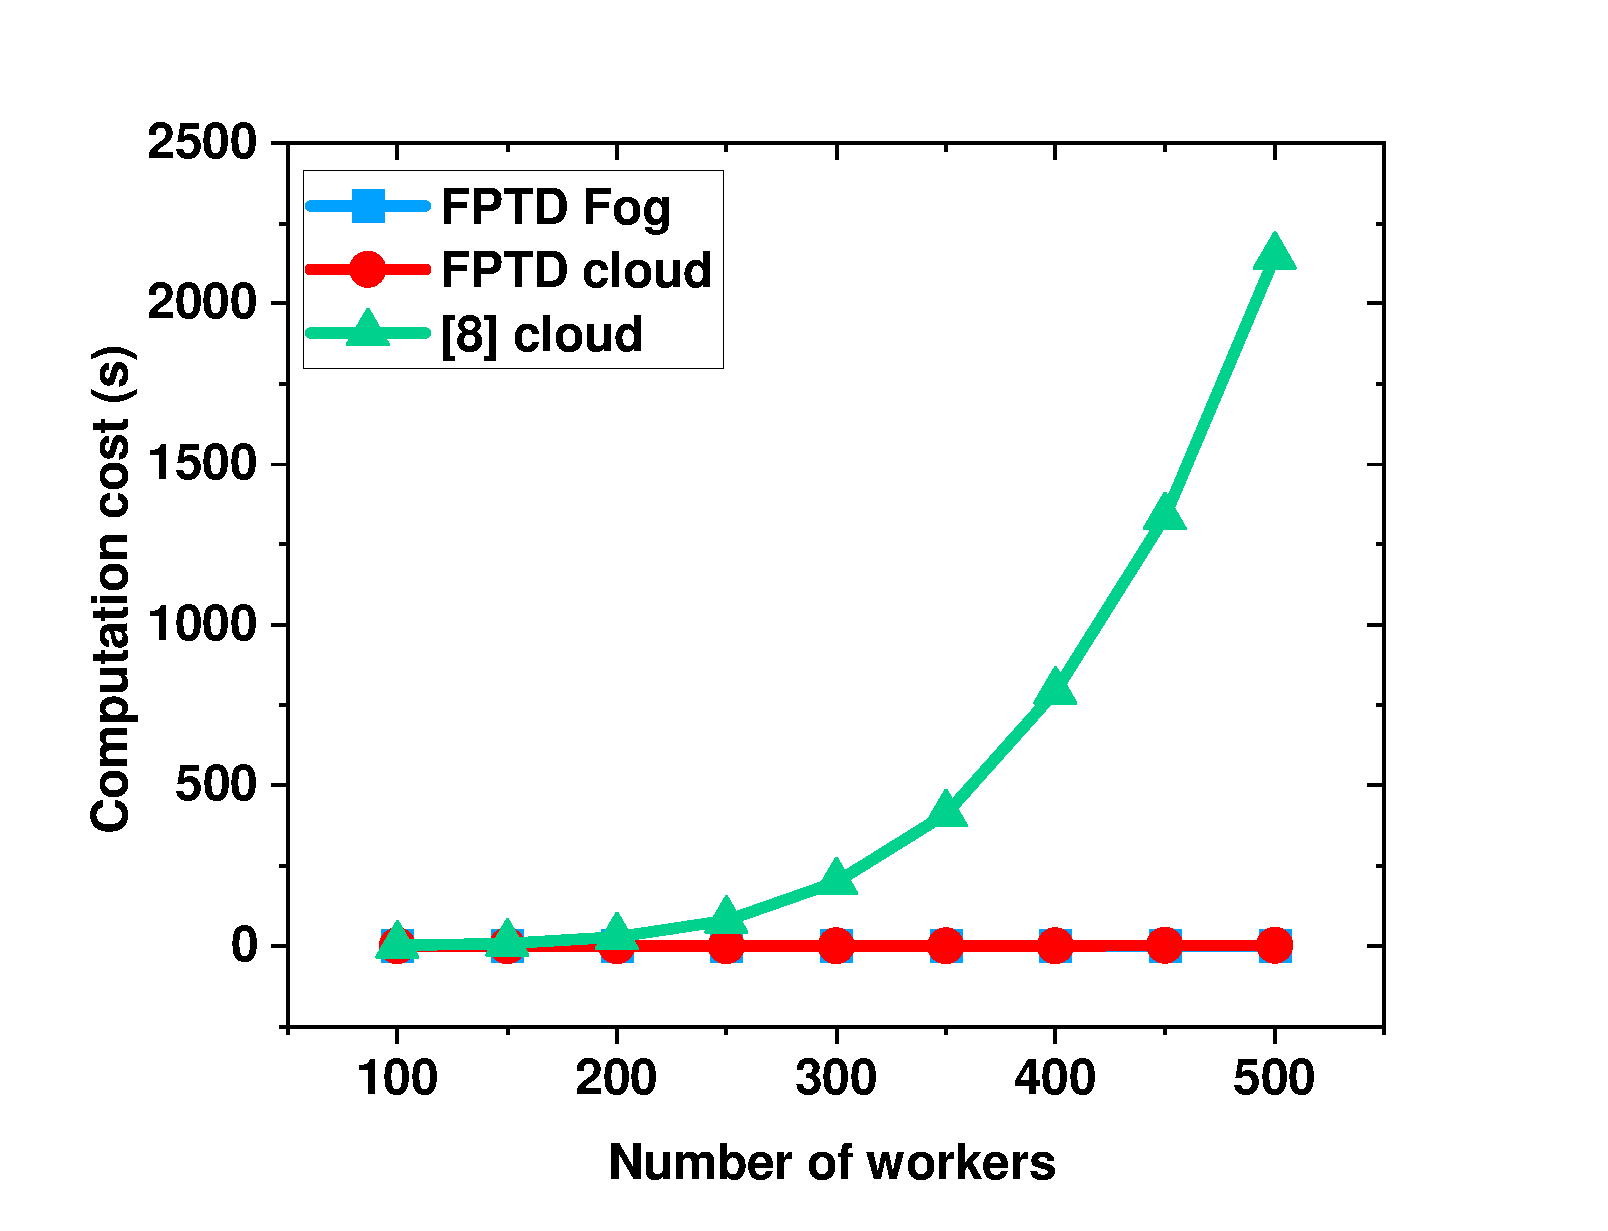
\includegraphics[width=0.50\linewidth]{pictures/varying_workers_server.pdf}}
        \caption{Average computation cost with varying workers}
        \label{workers}
    \end{figure}

    Next, we consider varying fog nodes which varies in range of $[1,2,3,4,5,6,10,15]$. The result is presented in Fig.\ref{fogs}. From Fig.\ref{fogs}, we can observe that when the number of fog nodes is set to only, i.e., one group, FPTD achieves similar efficiency as \cite{rtpt} with respect to all entities. Further, FPTD's computation overhead drops significantly when the number of fog nodes grows. However, there is a turning point after which the computation overhead drops slowly with respect to all entities. The above observations show that it is enough for FPTD to adopt only a few fog nodes to gain significant efficiency improvement.
    \begin{figure}[!ht]
        \centering
        \subfloat[Average time of workers]{
        \label{fogsa}
        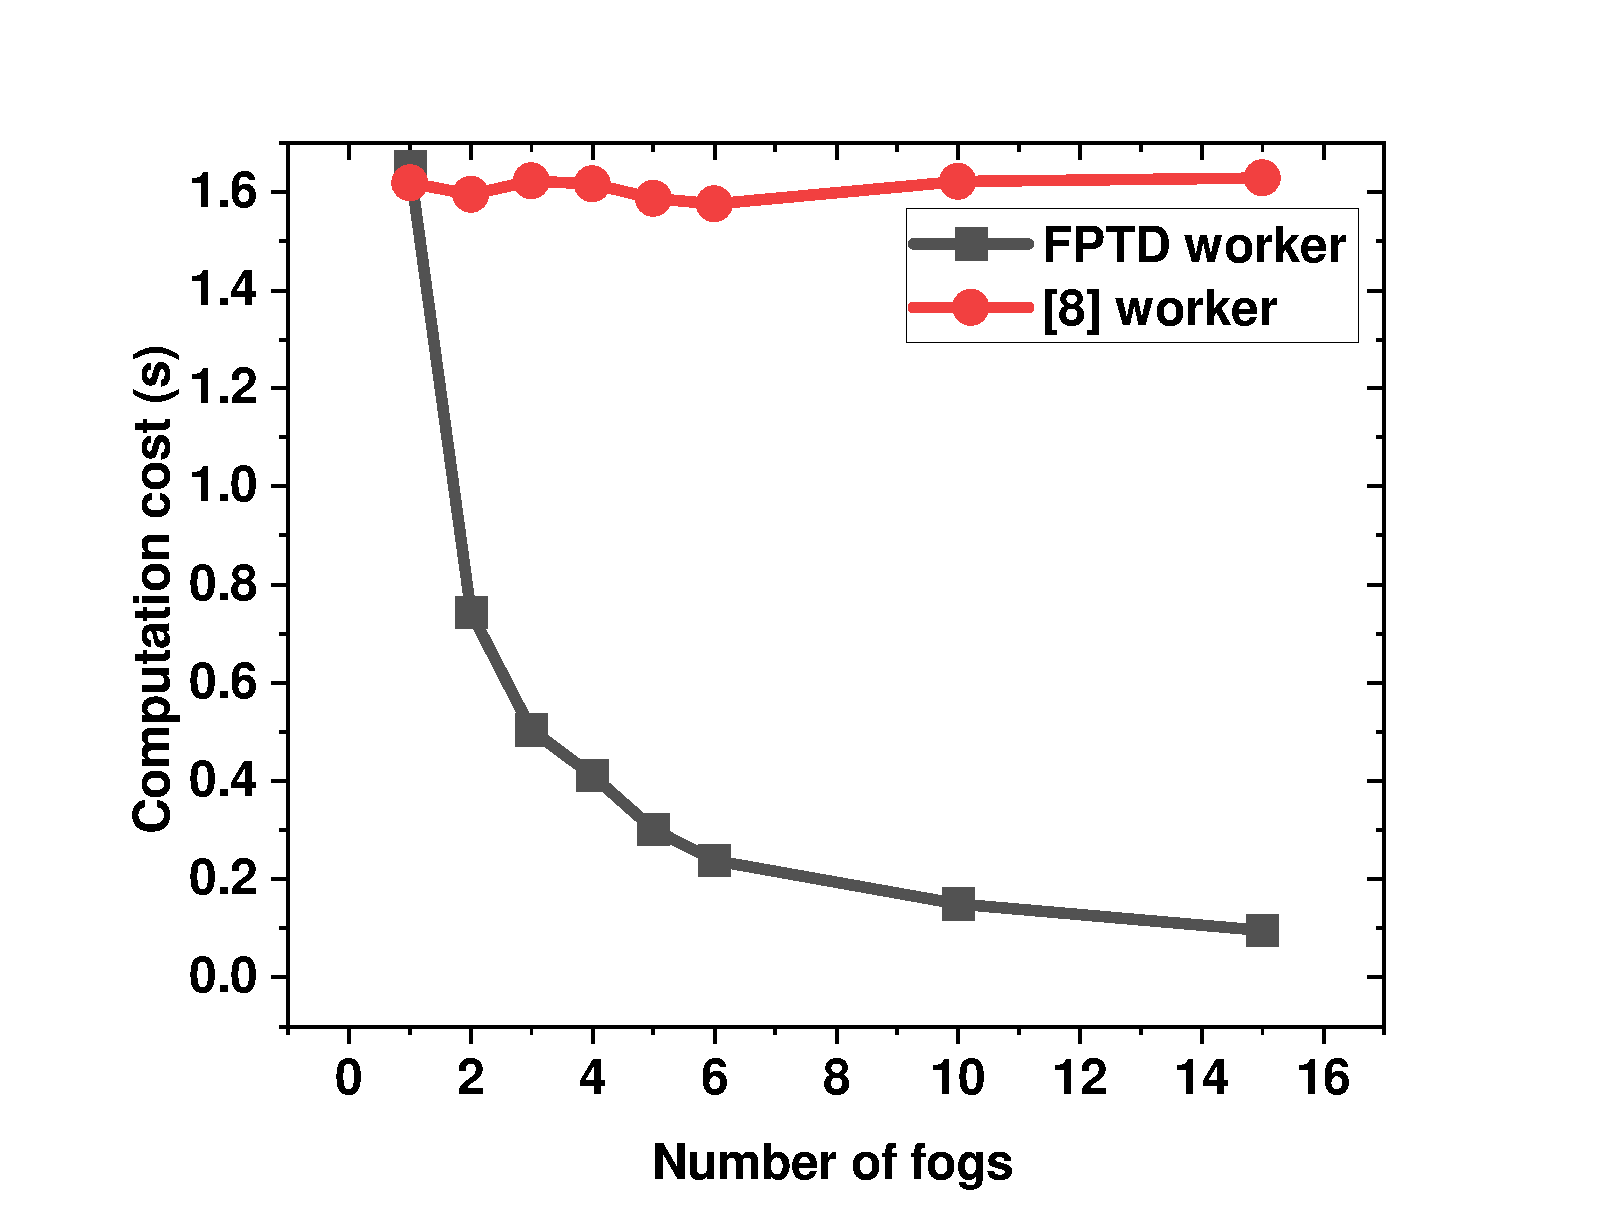
\includegraphics[width=0.48\linewidth]{pictures/varying_fog_worker.pdf}}
        \subfloat[Average time of cloud and fog]{
        \label{fogsb}
        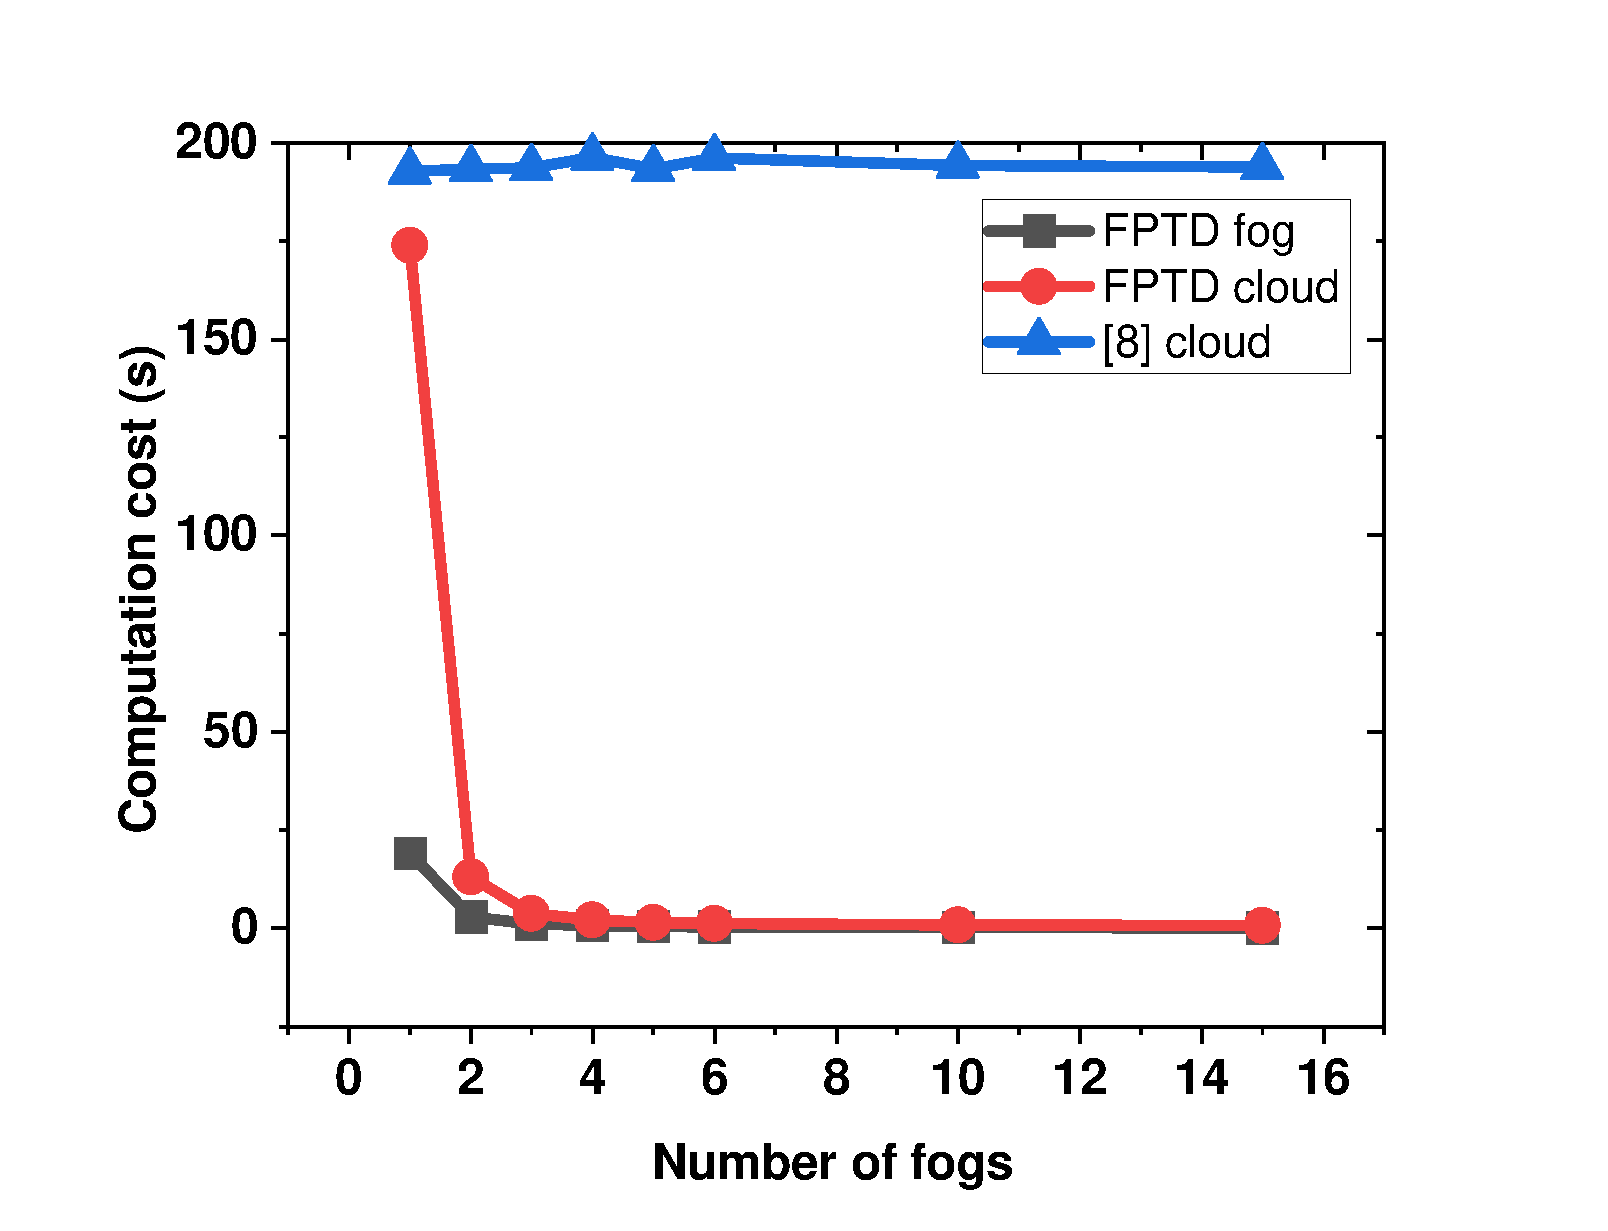
\includegraphics[width=0.48\linewidth]{pictures/varying_fog_server.pdf}}
        \caption{Average computation cost with varying fog nodes}
        \label{fogs}
    \end{figure}

    Finally, we consider the effect of the drop rate. Specifically, we let the drop rate vary from 0.00 to 0.20 by the stride of 0.05. Here we consider only workers' dropouts before submitting their masked input since this is the worst case which brings most computation and communication overheads. As shown in Fig.\ref{drop_ratea}, drop rate has little influence on worker's computation overhead since workers only need to upload shares of dropout workers. However, we can observe from Fig.\ref{drop_rateb} that the computation overhead of cloud of \cite{rtpt} and fog of FPTD grows linearly since they need to recover the secret keys of dropout workers to cancel the zero-sum mask. Besides, the cloud of FPTD's computation overhead drops since the cloud needs to recover fewer random masks.
    \begin{figure}[!ht]
        \centering
        \subfloat[Average time of workers]{
        \label{drop_ratea}
        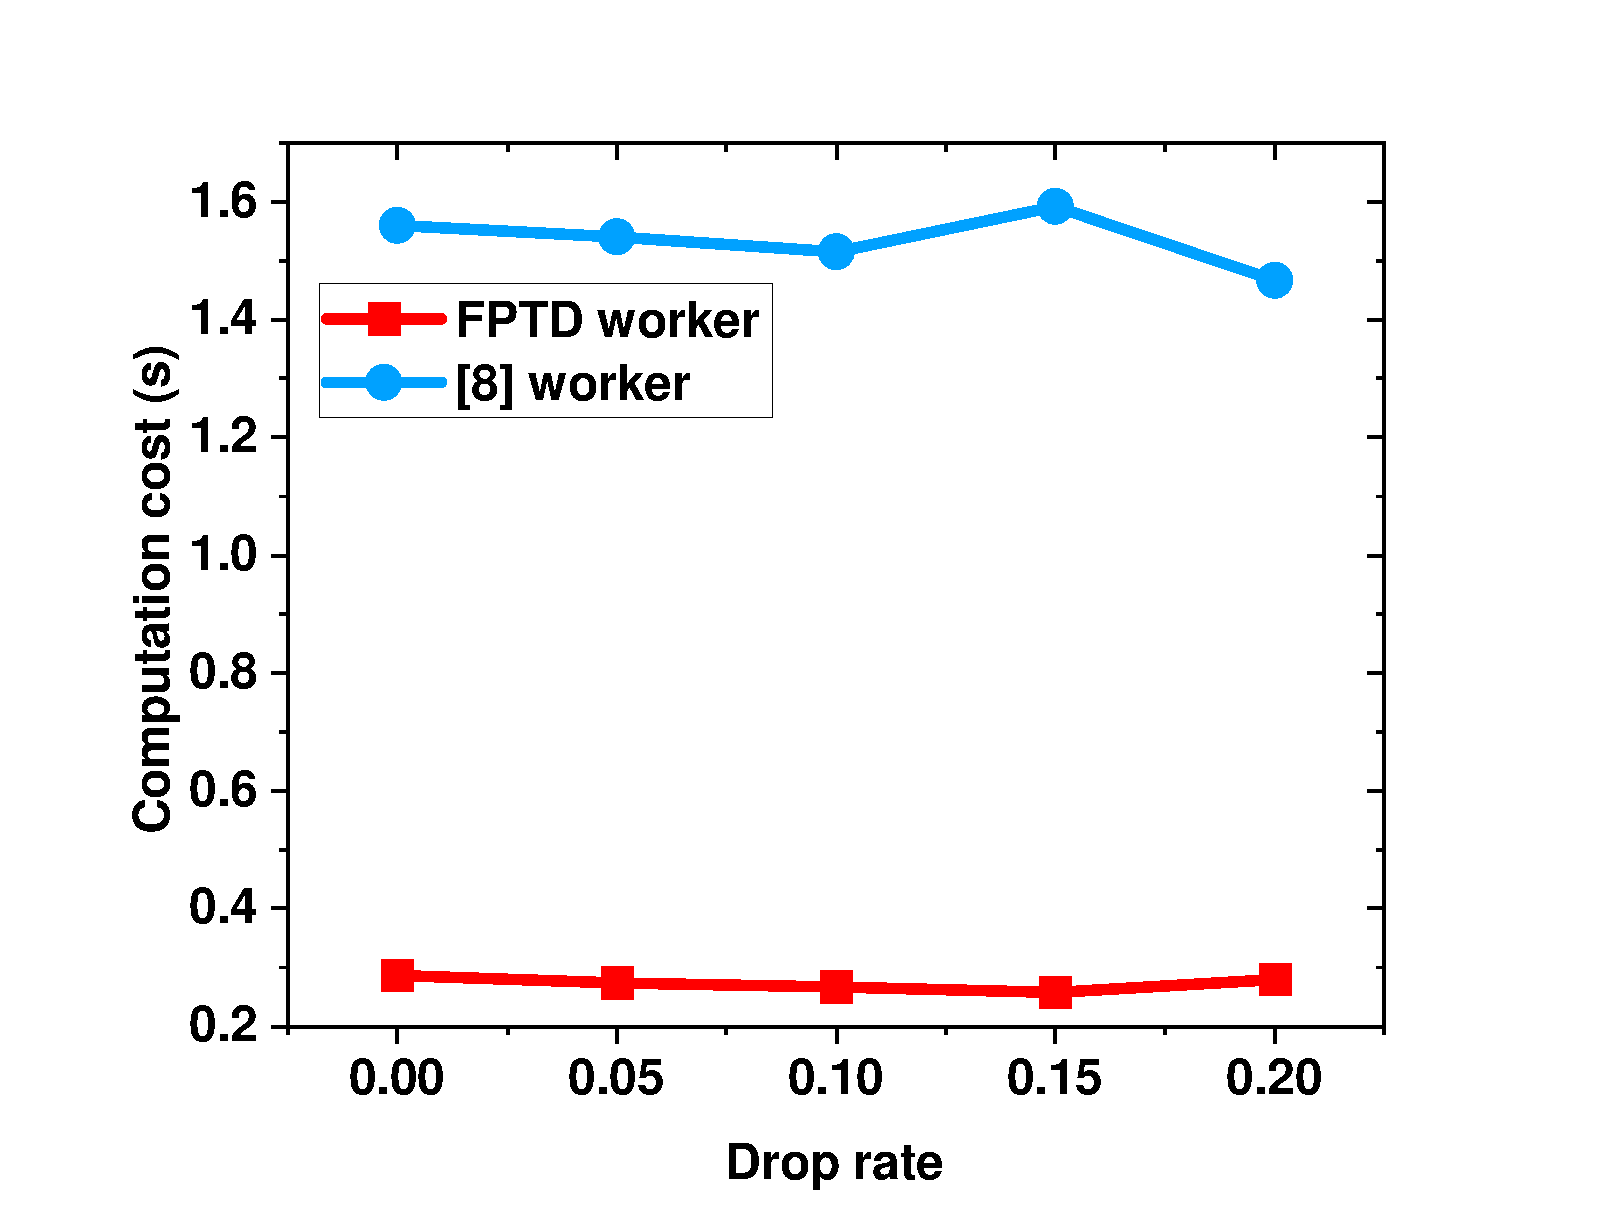
\includegraphics[width=0.44\linewidth]{pictures/varying_drop_rate_worker.pdf}}
        \subfloat[Average time of cloud and fog]{
        \label{drop_rateb}
        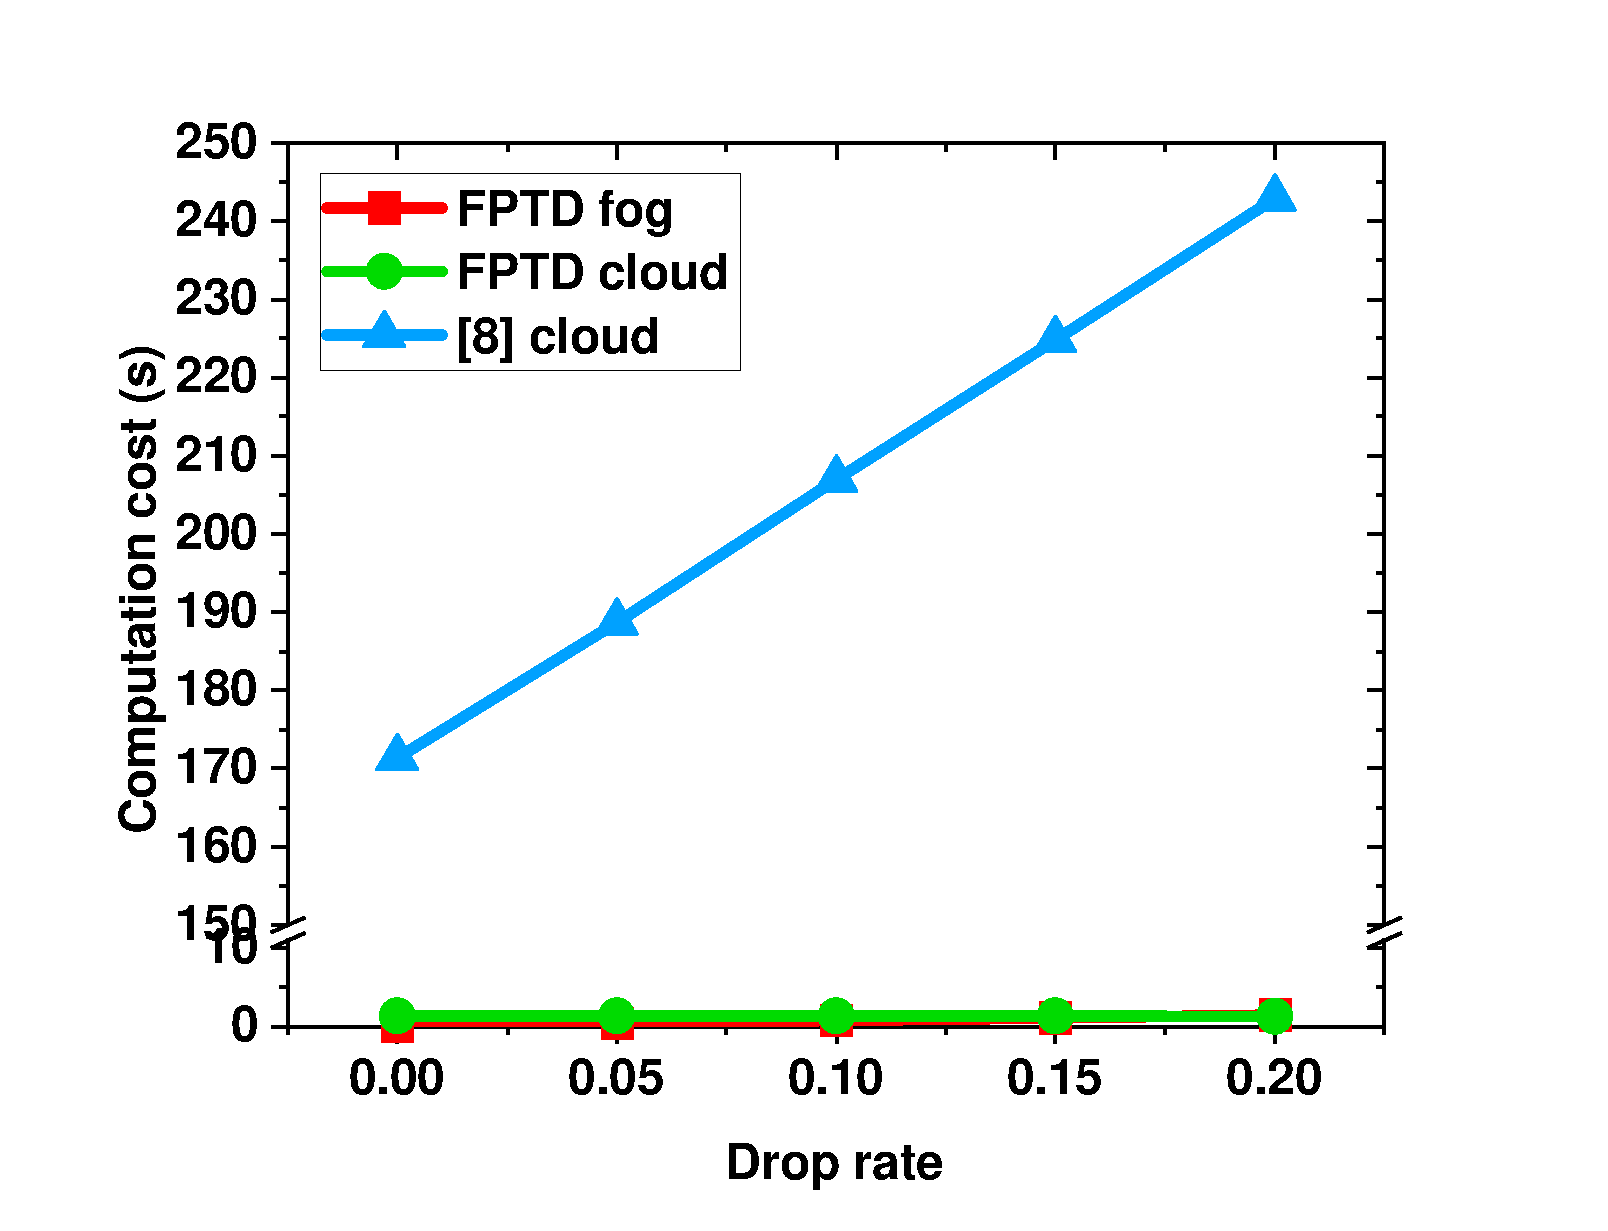
\includegraphics[width=0.45\linewidth]{pictures/varying_drop_rate_server.pdf}}
        \caption{Average computation cost with varying drop rate}
        \label{drop_rate}
    \end{figure}


    \subsection{Communication}
    In this part, we give performance comparisons between our FPTD and \cite{rtpt} in terms of communication overhead. First, we present the performance with varying number of workers. As illustrated in Fig.\ref{varying_worker_comm}, workers' communication costs of both FPTD and \cite{rtpt} grow linearly to the number of workers. However, our FPTD grows significantly slower than \cite{rtpt} since the group size of FPTD is divided by the number of fogs.
    \begin{figure}[!ht]
        \centering
        \subfloat[Average cost on each worker]{
        \label{varying_worker_comma}
        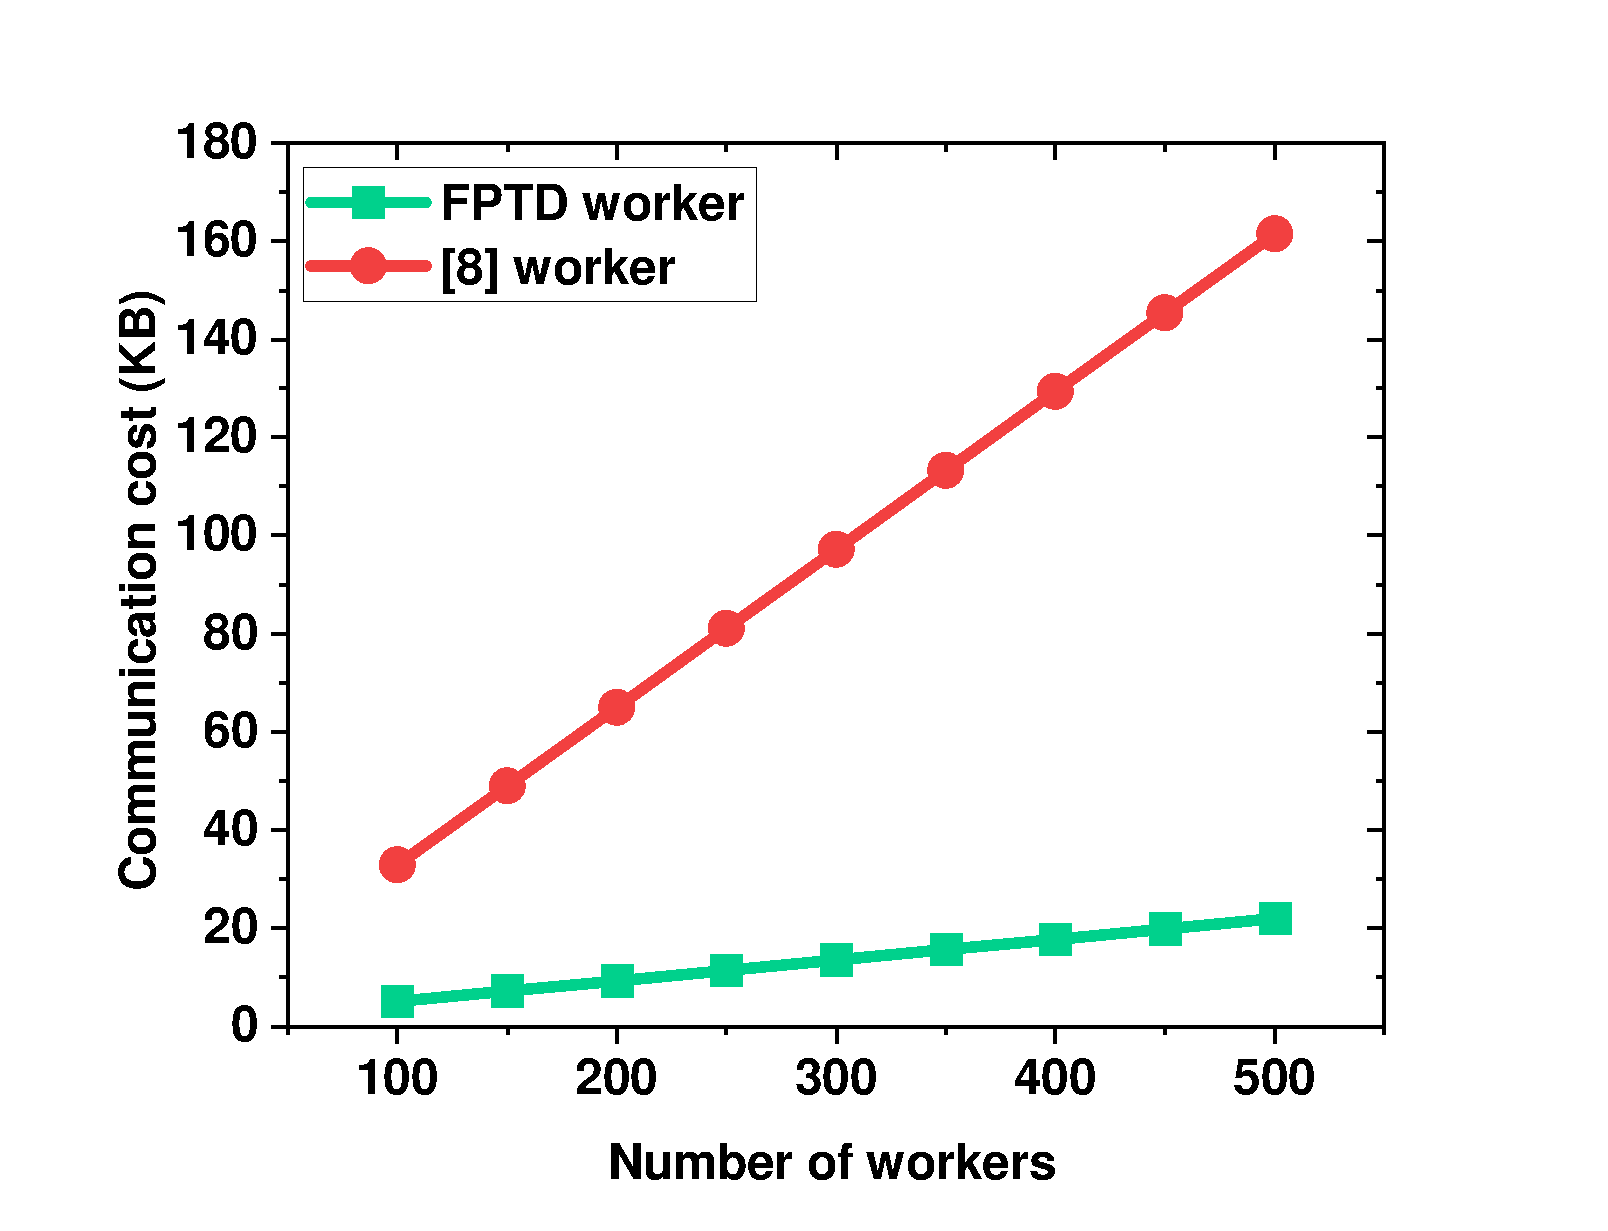
\includegraphics[width=0.48\linewidth]{pictures/varying_worker_worker_comm.pdf}}
        \subfloat[Average cost on cloud and fog]{
        \label{varying_worker_commb}
        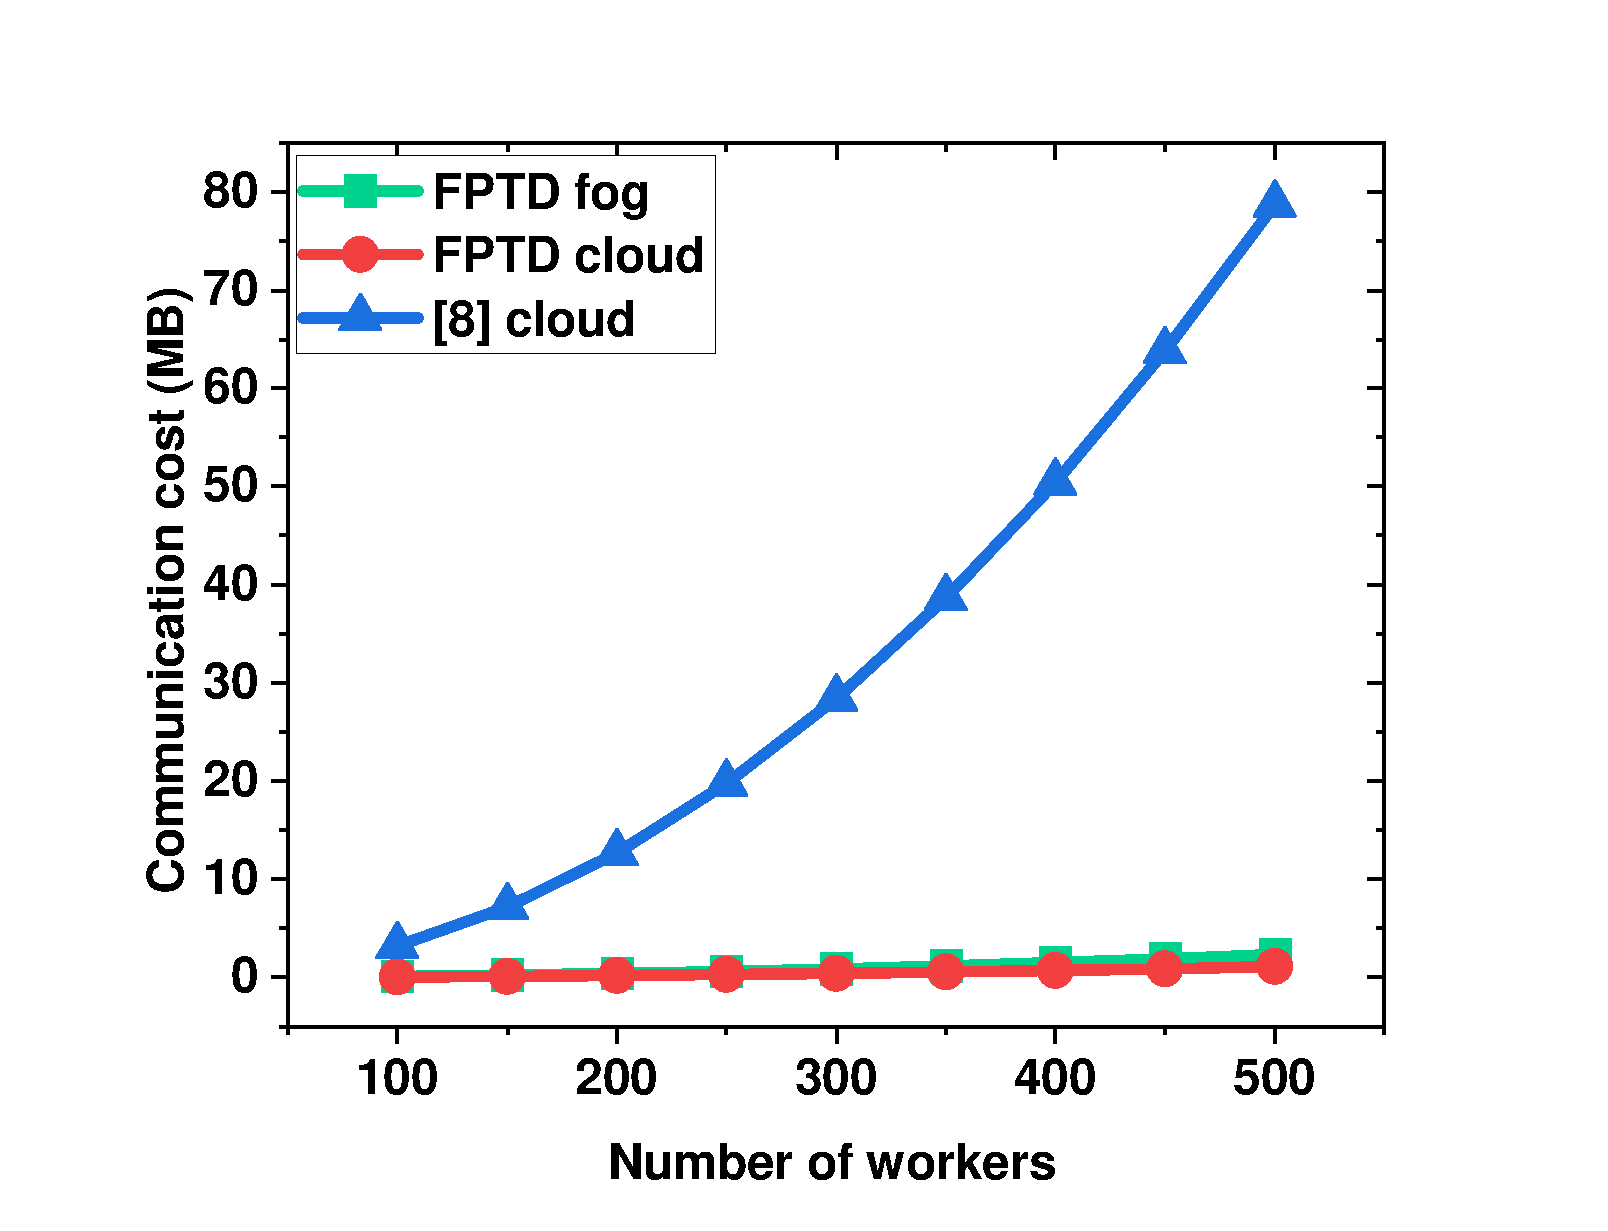
\includegraphics[width=0.48\linewidth]{pictures/varying_worker_server_comm.pdf}}
        \caption{Average communication cost with varying number of workers}
        \label{varying_worker_comm}
    \end{figure}

    Next, we compare the performance with a varying number of fog nodes. We can observe from Fig.\ref{varying_fog_comma} that the communication overhead of FPTD's workers drops when number of fog nodes grows. Moreover, the communication cost of FPTD's cloud is reduced since the cloud removes the burden of relaying the messages between workers. With more fog nodes, each fog node's communication overhead can also be significantly reduced since the group size is reduced.
    \begin{figure}[!ht]
        \centering
        \subfloat[Average cost on each worker]{
        \label{varying_fog_comma}
        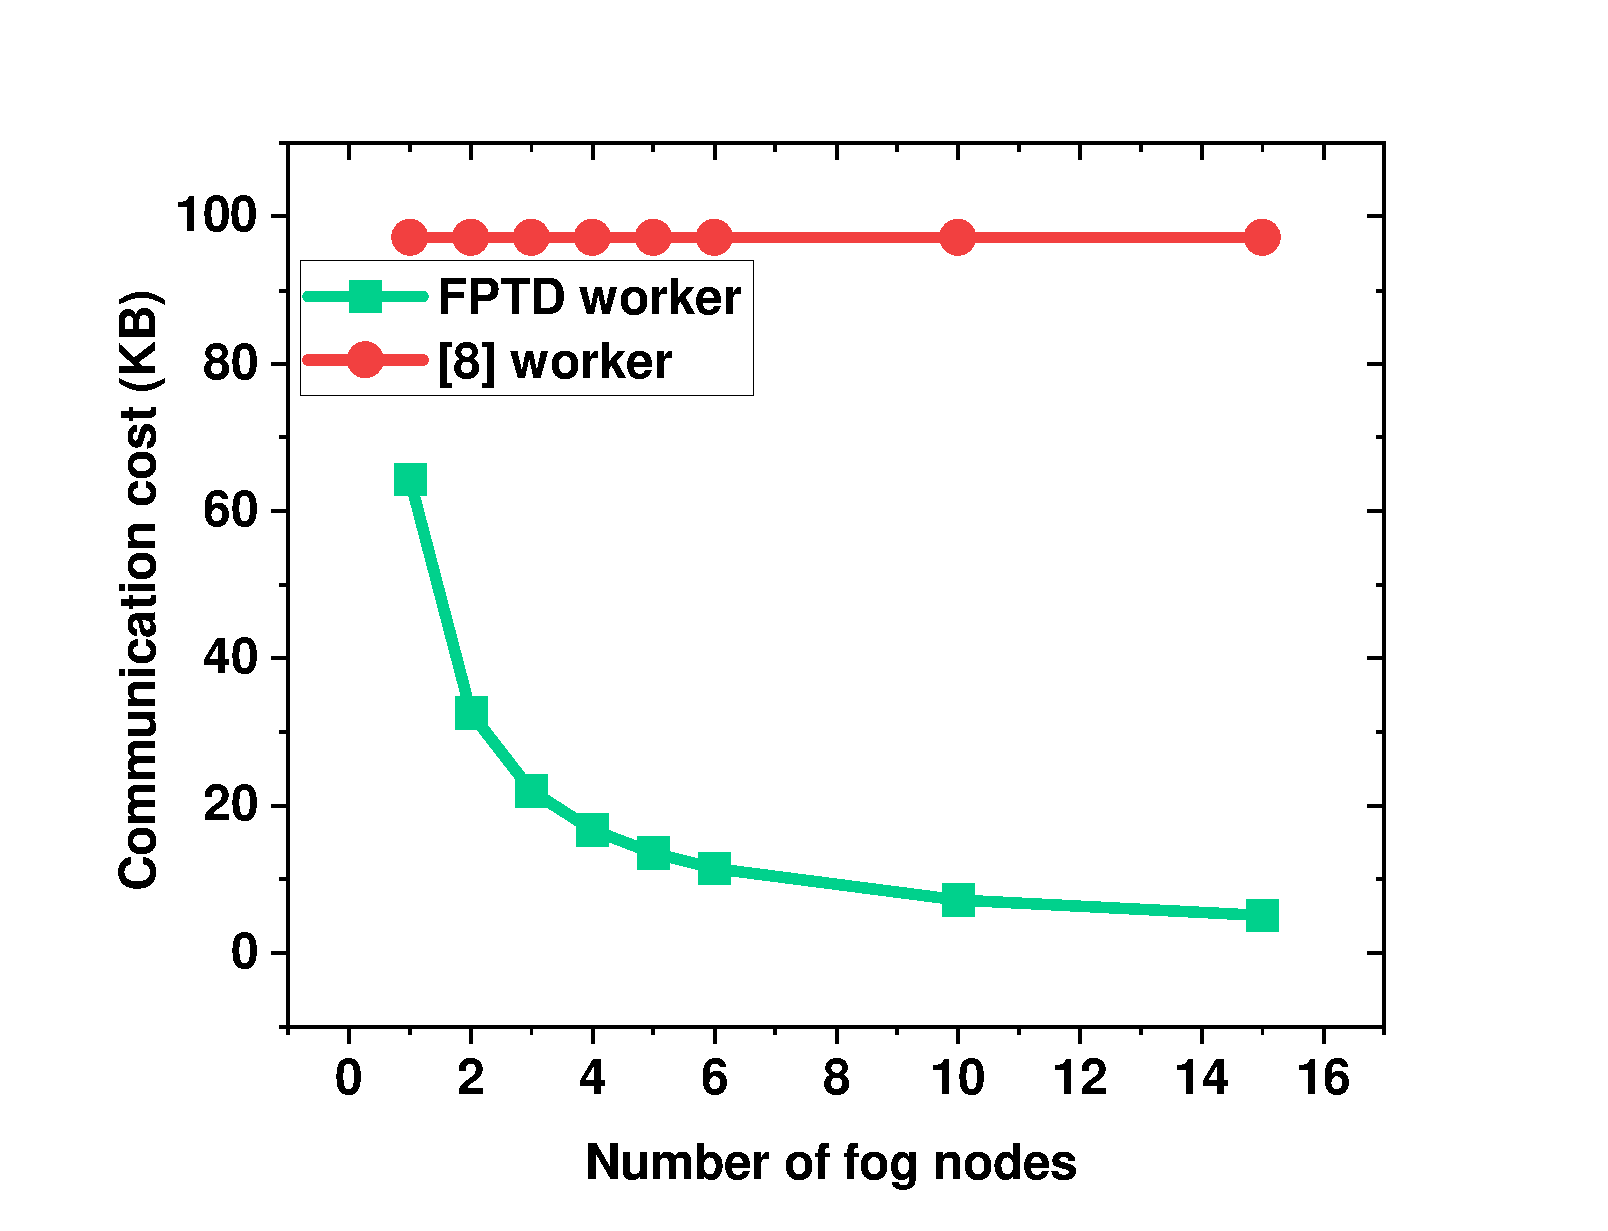
\includegraphics[width=0.48\linewidth]{pictures/varying_fog_worker_comm.pdf}}
        \subfloat[Average cost on cloud and fog]{
        \label{varying_fog_commb}
        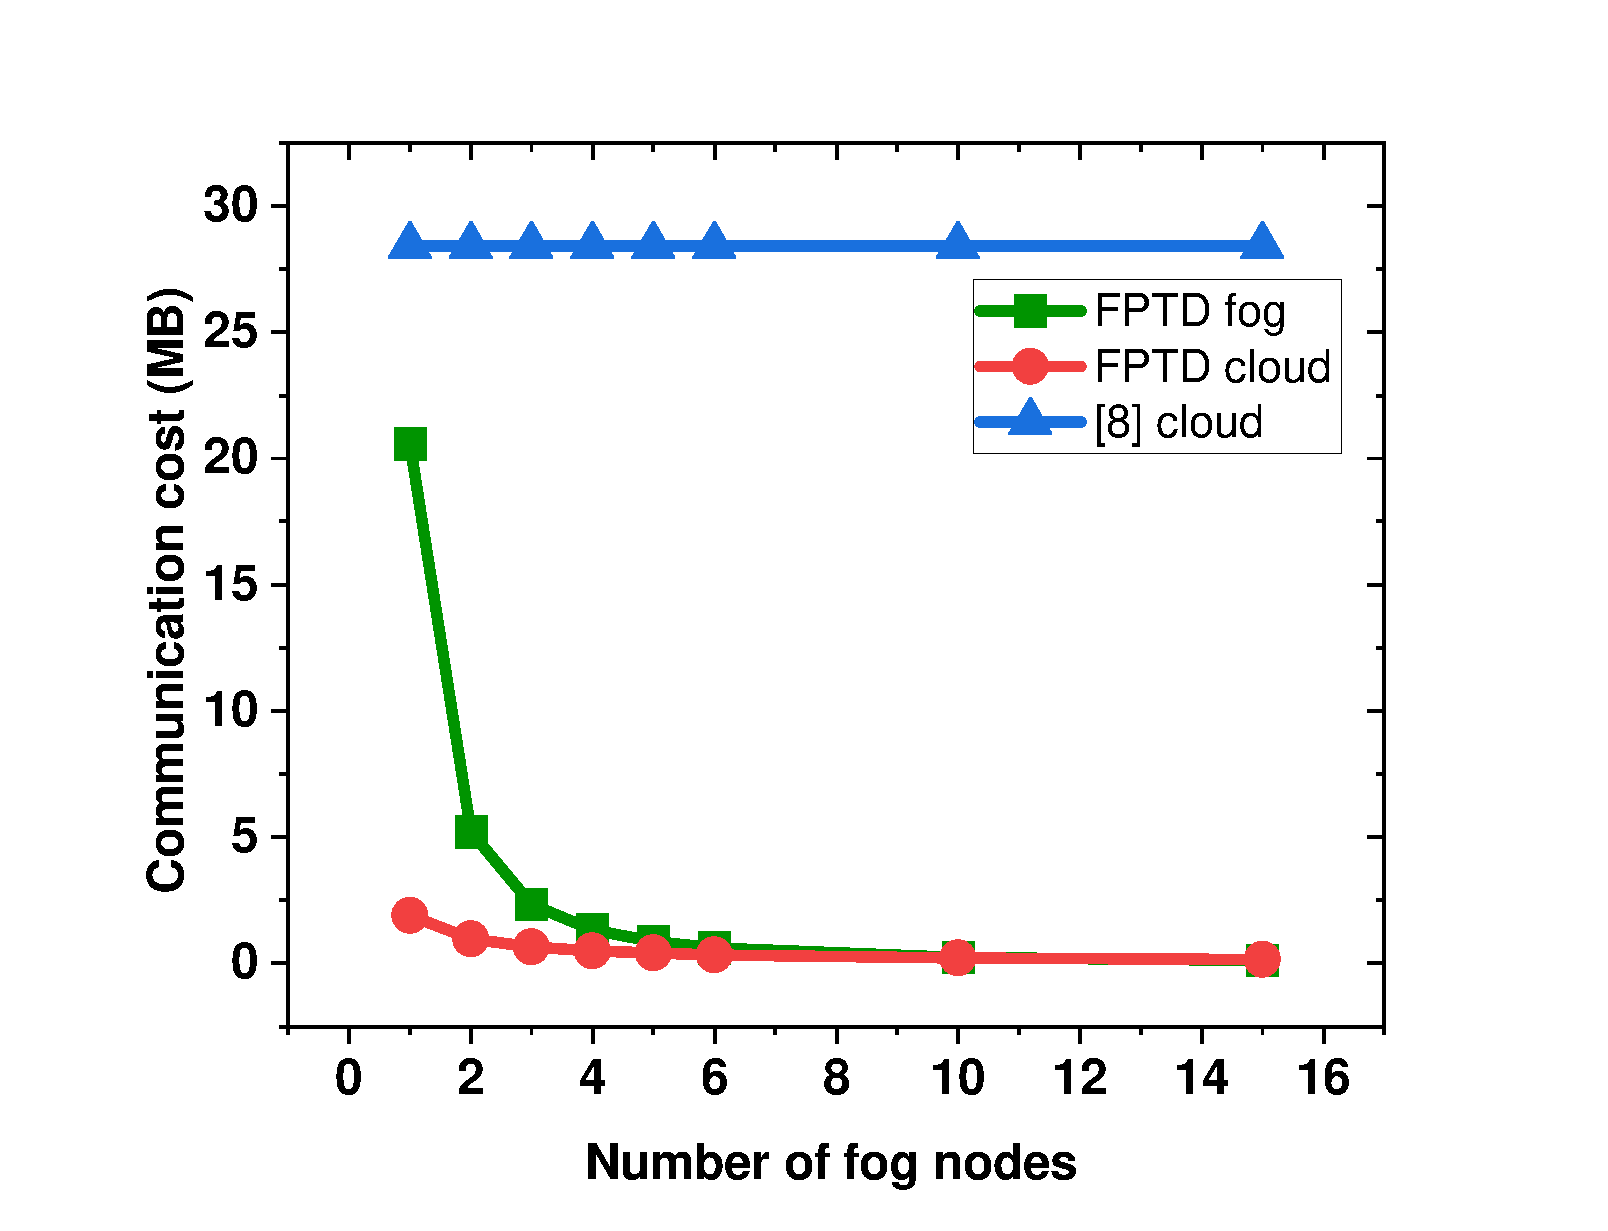
\includegraphics[width=0.48\linewidth]{pictures/varying_fog_server_comm.pdf}}
        \caption{Average communication cost with varying number of fogs}
        \label{varying_fog_comm}
    \end{figure}

    Due to space limitations, we omit the comparison with varying drop rates and varying objects since these two factors don't influence the communication overhead heavily.

\section{Conclusion}\label{conclusion}
%In this paper, we propose FPTD to address fog-aided privacy-preserving truth discovery in real-time applications. We design an improved PPTD scheme based on worker-fog-cloud architecture and we reach improvement on both efficiency and accuracy. We prove the security and conduct experiments to demonstrate that the proposed scheme is ideal for large-scale deployment.

In this paper, we propose FPTD, a privacy-preserving truth discovery framework for real-time applications in mobile crowdsensing system. Our FPTD can utilize fog nodes to divide the complete group into many small groups, which gains significant efficiency improvement in terms of both computation and communication. Besides, we design a much more efficient and failure-robust secure aggregation protocol which can aggregate results from these small groups with no privacy compromise. However, we leave specific group strategies as future directions.

\section*{Acknowledgment}
This work is supported in part by the National Natural Science Foundation of China under Grant No. 61972371 and Youth Innovation Promotion Association of the Chinese Academy of Sciences (CAS) under Grant No. Y202093.
\bibliographystyle{IEEETran}
\bibliography{main}
\end{document}
